\section{Analisi}
\label{sec:Analisi}


\subsection{Casi d'uso}
\label{sec:CasiDUso}
Per scoprire i requisiti del sistema, abbiamo evidenziato le interazioni fra utente e sistema mediante il grafico dei \emph{casi d'uso}:
\\
%\begin{figure}[!h]
%      \centering
      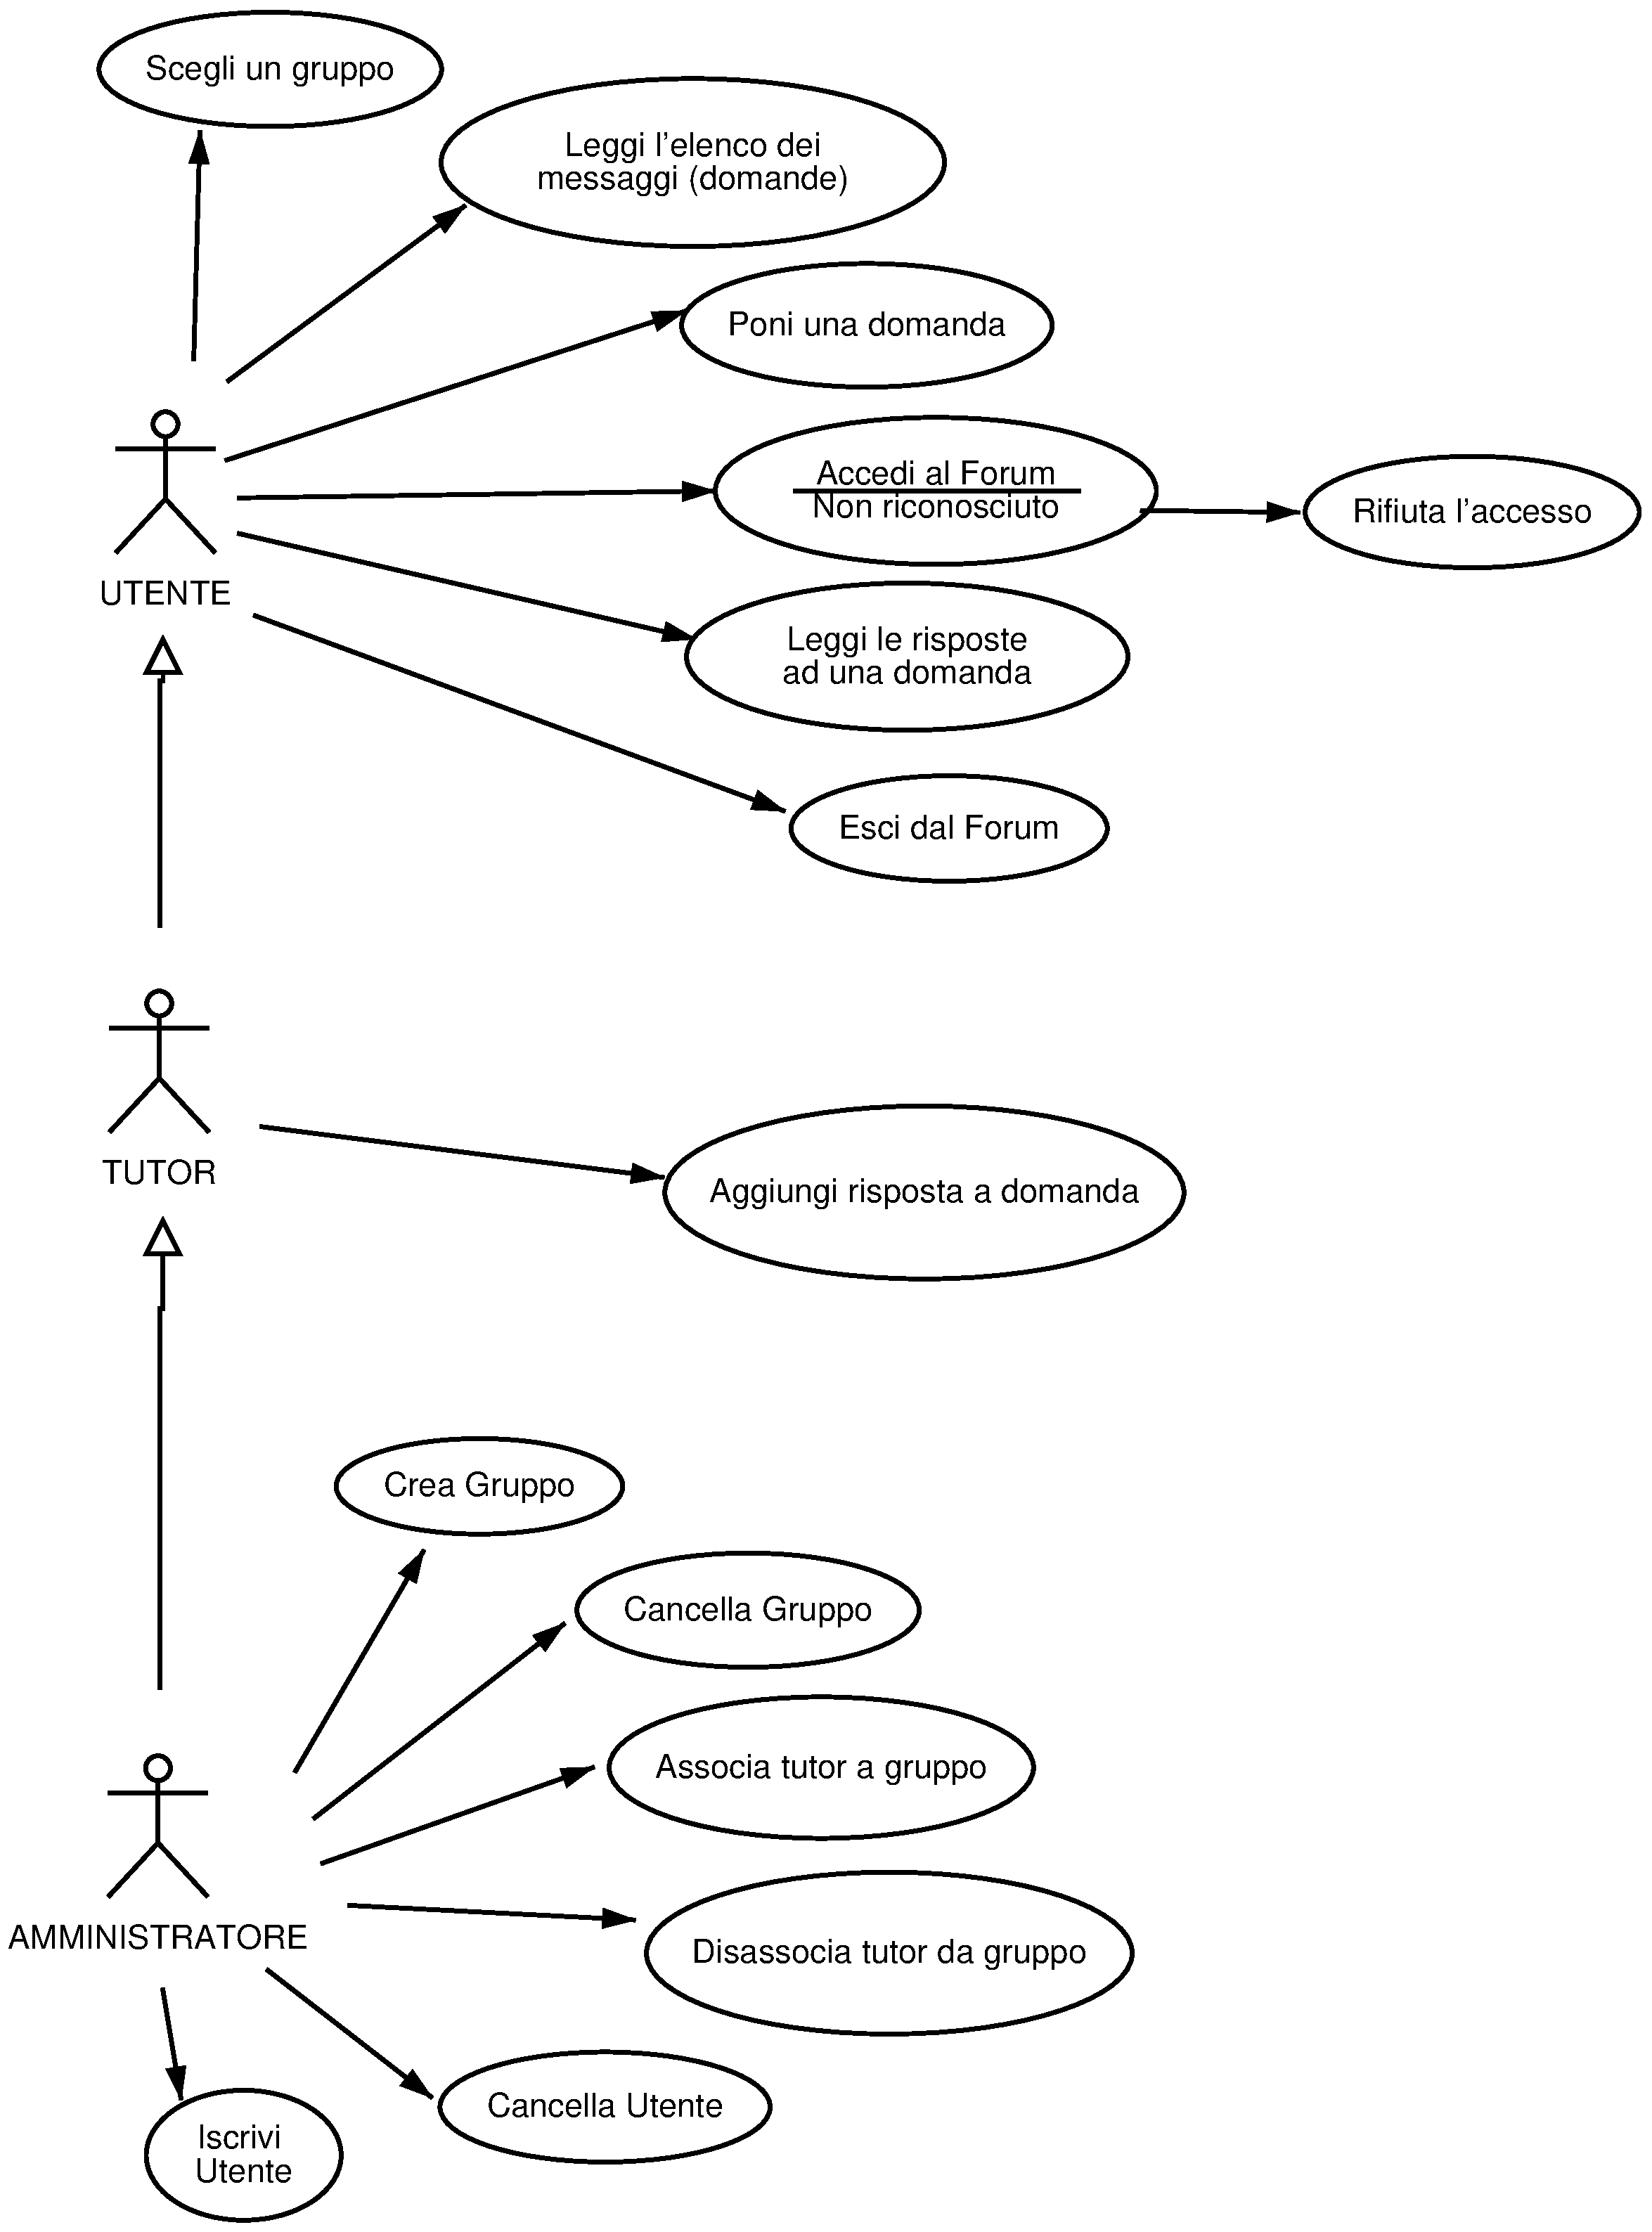
\includegraphics[angle = 0, width=\textwidth]{casiduso.eps}
%      \caption{Casi d'uso dell'applicazione}
%\end{figure}


\subsection{Specifiche dell'applicazione}
\label{sec:SpecificheDellApplicazione}

Dalla nostra analisi, sono derivate le seguenti specifiche:

Esistono tre tipi di utenti: Utente, Tutor, Amministratore.
Ogni utente � descritto dalle sue informazioni personali, pi� una login e una password per essere riconosciuto dal sistema.
Una volta entrato nel sistema, un utente semplice pu� accedere al forum, leggere le domande poste nei gruppi di discussione e porre nuove domande. 
I tutor sono degli utenti con la possibilit� di rispondere alle domande poste nei gruppi ai quali sono associati.
Gli amministratori sono tutor con la facolt� di:
\begin{itemize}
 \item aggiungere o cancellare gruppi di discussione del forum
 \item gestire le associazioni fra tutor e gruppi
 \item gestire le iscrizioni degli utenti
\end{itemize}

Se il sistema non possiede utenti, al suo avvio crea un amministratore con login "`root"' e password "`root"'. Questo primo utente creer� poi gli altri.